\documentclass[12pt,a4paper]{article}
\usepackage[margin=1in]{geometry}
\usepackage{setspace}
\doublespacing
\usepackage{amsmath,amssymb}
\usepackage{booktabs}
\usepackage{multirow}
\usepackage{float}
\usepackage{graphicx}
\usepackage[super]{natbib}
\usepackage{hyperref}
\hypersetup{hidelinks}
\usepackage{tikz}
\usetikzlibrary{positioning,arrows.meta,calc,decorations.pathreplacing}
\bibliographystyle{unsrtnat}

\title{Causal Transformer: Scaling Gradient-Based Causal Discovery with Self-Attention}

\author{Shuaidong Gao\thanks{Corresponding author. Chongqing Institute of Foreign Studies, Qijiang Campus, Chongqing 401420, China. E-mail: gaoshuaidong@stu.cqifs.edu.cn. ORCID: 0009-0004-5641-3581.}}

\date{\today}

\begin{document}

\maketitle

\begin{abstract}
NOTEARS dominates gradient-based DAG learning by optimizing each edge weight independently. We ask whether multi-head self-attention can instead construct the causal adjacency matrix, and introduce Causal Transformer (CT), which maps variable embeddings through attention into a signed, unbounded edge decoder under the NOTEARS acyclicity penalty. CT attains moderate structure recovery (F1 = 0.76 at d = 200, n = 1000) and its heads specialize into nearly disjoint variable-pair patterns (inter-head Jaccard 0.17). On 10 TCGA cancer types, CT's edges enrich in cancer-relevant genes (75% ClinGen Tier-1). Under identical metrics, NOTEARS attains higher F1 (0.98--0.99); CT's contribution is architectural.
\end{abstract}

\noindent\textbf{Keywords:} Causal discovery; Self-attention; Transformer; NOTEARS; DAG learning

\vspace{0.5em}

\section{Introduction}

Causal discovery---learning directed acyclic graphs (DAGs) from observational data---is a central problem in machine learning and systems biology \cite{zheng2018dags,sachs2005causal,peters2017elements}. NOTEARS \cite{zheng2018dags} recast DAG learning as continuous optimization with a smooth acyclicity constraint $h(W) = \mathrm{tr}(e^{W \odot W}) - d$; its cost is dominated by the $O(d^3)$ matrix exponential, so large $d$ remains expensive. We instead ask whether multi-head self-attention can build the adjacency matrix directly, so that each edge is informed by interactions across all variable pairs.

Real data often sit at this scale: the median MAD-filtered expression dimensionality across the 33 TCGA types is 198 genes, so $d=200$ is routine \cite{sporns2005human,heckerman1997bayesian}. Whether an attention-based constructor of $W$ works here, and whether it yields interpretable structure, is unexamined.

\textbf{Our contribution.} We introduce Causal Transformer (CT), which treats variables as tokens and learns causal edge weights from multi-head attention, decoding $W$ through a signed, unbounded map so that edge signs come from the decoder rather than the non-negative softmax. CT keeps NOTEARS' penalty $h(W)$ and is presented as an alternative attention-based DAG constructor, examined honestly.

\begin{enumerate}
    \item \textbf{Architecture.} A variable-as-token encoder maps an $n\times d$ matrix to a $d\times d$ adjacency matrix via multi-head attention under the NOTEARS penalty. Heads specialize into nearly disjoint interaction patterns (inter-head Jaccard $0.17$); edge signs are assigned separately by a signed, unbounded decoder.
    \item \textbf{Systematic characterization.} An 80-configuration sweep shows few meaningful edges below $d\approx100$ but trainable output at $d\ge200$; under standard metrics, official NOTEARS reaches higher F1, so CT's value is architectural.
    \item \textbf{Real-data operation.} CT sustains a non-zero output through $d=350$ on TCGA transcriptomic data, with an $O(d^2)$ memory ceiling near $d=500$. On 10 TCGA cancers at $d=200$, selected edges enrich in cancer-relevant genes (75\% of top hubs are ClinGen Tier-1), indicating biological plausibility.
\end{enumerate}

\section{Related Work}

CT sits at the intersection of differentiable causal discovery, Transformers for structured prediction, and multi-head specialization.

\subsection{Differentiable Causal Discovery}

The NOTEARS framework \cite{zheng2018dags} replaced combinatorial search with a smooth acyclicity penalty, enabling gradient-based DAG learning. Later work extended it to nonlinear SEMs (DAG-GNN \cite{yu2019daggnn}, Gran-DAG \cite{lachapelle2020gradient}), improved objectives (GOLEM \cite{ng2020golem}, DAGMA \cite{bello2022dagma}), and interventional \cite{brouillard2020differentiable} or time-series \cite{pamfil2020dynotears} settings.

NOTEARS variants differ in how $W$ is parameterized but all retain the acyclicity penalty. CT takes a different route: multi-head self-attention builds a feature representation of all variable pairs, which a signed, unbounded decoder maps to $W$, so each $W_{ij}$ receives gradient through all $d^2$ query--key pairs. We measure whether this construction is competitive on standard metrics (Section~\ref{sec:baseline_metrics}).

\subsection{Transformers for Structured Prediction}

The Transformer \cite{vaswani2017attention} has been adapted to structured prediction (Graph-BERT \cite{zhang2020graph}; Grover \cite{rong2020self}; SAN \cite{kreuzer2021rethinking}). CT differs in two ways: the graph is the \emph{output} rather than the input, and acyclicity is enforced explicitly via the penalty, distinguishing it from GNN-based causal models that encode graph structure in message passing.

\subsection{Multi-Head Specialization in Transformers}

Transformers commonly exhibit emergent head specialization. Clark et al. \cite{clark2019does} found BERT's heads specialize into syntactic roles (inter-head Jaccard as low as 0.12). CT shows an analogous phenomenon: its heads attend to largely disjoint variable-pair sets (Jaccard $0.17$; Section~\ref{sec:head_spec}), while edge sign is assigned by the signed decoder (Eq.~\ref{eq:signed_decoder}) rather than by any single head. This separation of head-level attention and decoder-level sign assignment has not, to our knowledge, been characterized in causal discovery.

\subsection{Attention-Based Causal Discovery}

DAG-Transformer \cite{lorch2022gadget} and A-DAG \cite{ke2023learning} use attention for \emph{variable ordering}, decoding DAGs by sequential regression on small graphs ($d<50$). CT instead uses attention to provide the interaction features, which a signed, unconstrained decoder maps directly to the adjacency matrix with no ordering step; the resulting $W$ is regularized to be a DAG (Eq.~\ref{eq:signed_decoder}). This avoids the ordering search and lets CT train at $d=200$--$500$ on consumer hardware.

\subsection{Graph Attention for Biological Network Reconstruction}

Graph attention has also reconstructed biological \emph{topology}: GAT-HiC \cite{kaya2026gathic} recovers 3D chromosome structure and BioCode \cite{sefer2022biocode} models network growth. CT shares this architectural spirit but differs in objective: these methods reconstruct an observed topology, whereas CT \emph{infers} a directed acyclic structure while enforcing acyclicity.

\subsection{Mid-Scale Motivation}

Small-$d$ methods are constraint-based (PC; \cite{spirtes2000causation}), score-based (GES; \cite{chickering2002optimal}), or hybrid (LiNGAM; \cite{shimizu2006lingam}); large-$d$ methods use low-rank factorization \cite{chen2023lowrank} or divide-and-conquer \cite{gu2022large}. Deep-learning causal-effect models \cite{makala2026causal} target prediction rather than structure recovery. CT is an attention-based gradient DAG learner trainable at $d=200$--$500$ on consumer hardware; we make no claim of superior accuracy, assessed separately in Section~\ref{sec:std_metrics}.

\section{Methods}

\subsection{Causal Transformer Architecture}

Figure~\ref{fig:architecture} provides a schematic overview.

% --- TikZ architecture diagram ---
\definecolor{CTc}{HTML}{1F5C8B}
\definecolor{NOTc}{HTML}{B4513C}
\definecolor{INKc}{HTML}{1A1A1A}
\definecolor{CINPUT}{HTML}{E9F2E9}
\definecolor{CEMBED}{HTML}{DDEBF7}
\definecolor{CATTN}{HTML}{FDF2E3}
\definecolor{CAGG}{HTML}{E3F0E4}
\definecolor{CDAG}{HTML}{FBE4DF}
\definecolor{COUT}{HTML}{EDE6F5}
\definecolor{CBORD}{HTML}{333333}
\definecolor{CARROW}{HTML}{4A4A4A}
\definecolor{HLOSS}{HTML}{FBF0DC}
\definecolor{HLOSSBD}{HTML}{C9A15A}
\definecolor{TXTSUB}{HTML}{555555}
\definecolor{TXTGRAY}{HTML}{8A5A00}
\definecolor{H1}{HTML}{1F5C8B}
\definecolor{H2}{HTML}{38709A}
\definecolor{H3}{HTML}{4F81AD}
\definecolor{H4}{HTML}{6B97B8}
\definecolor{H5}{HTML}{85ABC7}
\definecolor{H6}{HTML}{9EBED7}
\definecolor{H7}{HTML}{B8D2E6}
\definecolor{H8}{HTML}{D1E6F5}

\begin{figure}[htbp]
\centering
\begin{tikzpicture}[
  font=\scriptsize,
  nbox/.style={draw=CBORD, line width=1.0, rounded corners=2.5pt, align=center,
               inner sep=5pt, text width=3.5cm, minimum height=1.5cm},
  wbox/.style={draw=CBORD, line width=0.8, rounded corners=3pt, align=left,
               inner sep=6pt, text width=3.5cm, fill=white},
  head/.style={draw=CBORD, line width=0.6, rounded corners=1.5pt,
               minimum width=1.0cm, minimum height=0.46cm, align=center},
  ar/.style={-{Stealth[length=2.4mm]}, color=CARROW, line width=1.2},
  bg/.style={draw=CBORD, line width=1.0, rounded corners=2.5pt,
             fill=CATTN, inner sep=0pt, minimum height=5.4cm, minimum width=7.4cm},
]
% Title
\node[font=\large\bfseries, color=INKc] (TITLE) {Causal Transformer (CT) Architecture};
% Stem (all relative -> no overlap)
\node[nbox, fill=CINPUT, below=0.7cm of TITLE] (IN)
  {Input Data Matrix\\[1pt]\scriptsize $X\in\mathbb{R}^{n\times d}$};
\node[nbox, fill=CEMBED, below=0.55cm of IN] (EM)
  {Variable Embedding\\[1pt]\scriptsize $E_i = X_{:,i}\,W_{\text{embed}}$\\
   \textcolor{TXTSUB}{\scriptsize $E\in\mathbb{R}^{d\times d_{\text{model}}}$}};
\draw[ar] (IN.south) -- node[left, pos=0.5]{per-variable} (EM.north);
% Attention container
\node[bg, below=0.55cm of EM] (ATTN) {};
\node[font=\bfseries, color=INKc] (AN) at ($(ATTN.center)+(0,2.05)$) {Multi-Head Self-Attention};
\node[font=\scriptsize, color=INKc, align=center] (AE) at ($(ATTN.center)+(0,1.32)$)
  {$A^{(h)}=\mathrm{softmax}\!\Big(\frac{(EW_Q^{(h)})(EW_K^{(h)})^\top}{\sqrt{d_k}}\Big)$};
\foreach \i/\xx/\hh in {1/-2.4/H1, 2/-0.8/H2, 3/0.8/H3, 4/2.4/H4}
  \node[head, fill=\hh] (h\i) at ($(ATTN.center)+(\xx,0.55)$) {H\i};
\foreach \i/\xx/\hh in {5/-2.4/H5, 6/-0.8/H6, 7/0.8/H7, 8/2.4/H8}
  \node[head, fill=\hh] (h\i) at ($(ATTN.center)+(\xx,-0.15)$) {H\i};
\node[text width=6.9cm, align=center, font=\scriptsize, color=TXTGRAY] (HN) at ($(ATTN.center)+(0,-1.55)$)
  {\textbf{Head specialization:} heads attend to nearly disjoint variable-pair sets\\
   (inter-head Jaccard $0.17$); edge sign is assigned by the signed decoder};
\draw[ar] (EM.south) -- node[left, pos=0.5]{split} (ATTN.north);
% Side panels
\node[wbox, left=1.0cm of ATTN] (KI)
  {\textbf{Key Innovations}\\[3pt]
   \scriptsize No positional encoding\\ Permutation-invariant\\ 8 specialized heads\\
   \textcolor{TXTGRAY}{\bfseries $\to$ Signed edge decoder}\\ DAG penalty $h(W)$\\
   Pairwise $d^2$ gradient signals};
\node[wbox, draw=HLOSSBD, line width=1.0, fill=HLOSS, right=2.4cm of ATTN] (LOSS)
  {\textbf{Total Loss}\\[3pt]
   \scriptsize $\mathcal{L}=\frac{1}{2n}\|X-XW\|_F^2$\\[1pt]
   \scriptsize ${}+\lambda_1\|W\|_1+\frac{\rho}{2}h(W)^2$};
% Bottom row (DAG centred -> balanced)
\node[nbox, fill=CDAG, below=1.1cm of ATTN] (DAG)
  {\textbf{DAG Constraint}\\[1pt]\scriptsize $h(W)=\mathrm{tr}\!\left(e^{W\odot W}\right)-d$};
\node[nbox, fill=CAGG, left=1.5cm of DAG] (DEC)
  {\textbf{Signed Edge Decoder}\\[1pt]\scriptsize $W=g(\mathrm{vec}(\bar{A}))$\\
   \textcolor{TXTSUB}{\scriptsize $g:\mathbb{R}^{d^2\to256\to d^2}$}};
\node[nbox, fill=COUT, right=1.5cm of DAG] (OUT)
  {\textbf{Causal Graph}\\[1pt]\scriptsize $\widehat{W}$ (acyclic DAG)};
% Attention -> pool -> Decoder
\draw[ar] (ATTN.south) -- ++(0,-0.55) coordinate (p) -- (p -| DEC.north) -- (DEC.north);
\node[font=\scriptsize, color=TXTSUB, anchor=south, yshift=0.03cm]
  at ($(p)!0.5!(p-|DEC.north)$) {pool heads $\to\bar{A}\to g$};
% DEC -> DAG -> OUT
\draw[ar] (DEC.east) -- (DAG.west);
\node[font=\scriptsize, color=TXTSUB, anchor=south, yshift=0.11cm]
  at ($(DEC.east)!0.5!(DAG.west)$) {enforce};
\draw[ar] (DAG.east) -- (OUT.west);
\node[font=\scriptsize, color=TXTSUB, anchor=south, yshift=0.11cm]
  at ($(DAG.east)!0.5!(OUT.west)$) {acyclic};
% OUT -> Total Loss
\draw[ar] (OUT.north) -- (LOSS.south);
% Total Loss -> attention (dashed red back-prop)
\draw[-{Stealth[length=2.4mm]}, color=NOTc, line width=1.8, dashed]
  (LOSS.west) -- (ATTN.east);
\node[font=\scriptsize, color=NOTc, anchor=north, align=center]
  at ($(LOSS.west)!0.5!(ATTN.east)$) {gradient\\ $\partial\mathcal{L}/\partial Q,K$};
\end{tikzpicture}
\caption{\textbf{CT architecture.} Variables are embedded into $d_{\text{model}}$-dimensional tokens and processed through 8-head self-attention. The non-negative attention matrices are pooled across heads and layers into a representation $\bar{A}$, which a signed, unconstrained decoder $g$ maps to the causal adjacency matrix $W$ (so edge signs come from $g$, not from the softmax). $W$ is regularized by the DAG constraint $h(W)$. The total loss combines reconstruction error, L1 sparsity, and the augmented Lagrangian acyclicity penalty. The dashed red arrow indicates gradient backpropagation through all $Q,K$ pairs, providing $d^2$ pairwise gradient pathways that distinguish CT from NOTEARS.}
\label{fig:architecture}
\end{figure}


CT treats each variable $i$ as a token. The input is the transposed matrix $X \in \mathbb{R}^{n \times d}$ ($n$ samples, $d$ variables).

\textbf{Variable embedding.} Each variable $i$ is embedded via a learned linear projection followed by sample-wise averaging:
\begin{equation}
    E_i = \frac{1}{n} \sum_{k=1}^{n} (X_{k,i} \cdot W_{\text{embed}}) \in \mathbb{R}^{d_{\text{model}}}
    \label{eq:embedding}
\end{equation}
where $W_{\text{embed}} \in \mathbb{R}^{1 \times d_{\text{model}}}$ is shared across all variables. The $d$ resulting embeddings $E \in \mathbb{R}^{d \times d_{\text{model}}}$ form the token sequence input to the attention layers.

\textbf{Multi-head self-attention.} The $d$ stacked embeddings are projected into queries and keys via learned weight matrices $W_Q^{(h)}, W_K^{(h)} \in \mathbb{R}^{d_{\text{model}} \times d_k}$ for each head $h$:
\begin{equation}
    A^{(h)} = \text{softmax}\left(\frac{(E W_Q^{(h)})(E W_K^{(h)})^\top}{\sqrt{d_k}}\right)
    \label{eq:per_head}
\end{equation}
where $d_k = d_{\text{model}} / n_{\text{heads}}$. The softmax gives $A^{(h)} \in \mathbb{R}^{d \times d}$, where $A_{ij}^{(h)}$ is the attention variable $i$ pays to variable $j$. Each $A^{(h)}$ is a non-negative, row-stochastic \emph{attention} matrix encoding an interaction representation; it is \emph{not} the causal graph and is not constrained to be lower-triangular---acyclicity is enforced by the penalty rather than by architecture.

\textbf{Signed edge decoder.} The attention matrices are feature representations, not edge weights. Because softmax is non-negative, a separate signed, unconstrained decoder maps the pooled attention to the graph. We average $A^{(h)}$ across heads and layers to form $\bar{A}\in\mathbb{R}^{d\times d}$, then apply a two-layer MLP $g$ with no bounded activation:
\begin{equation}
    W = g\left(\mathrm{vec}(\bar{A})\right), \qquad g = \mathrm{Linear}_{d \times d \to 256} \circ \mathrm{ReLU} \circ \mathrm{Linear}_{256 \to d \times d}
    \label{eq:signed_decoder}
\end{equation}
where $W\in\mathbb{R}^{d\times d}$. The terminal layer of $g$ has no sigmoid or softmax, so its weights and bias take both positive and negative values; the sign of $W_{ij}$ encodes the direction of the effect variable $i$ exerts on $j$. Attention thus builds non-negative features and the decoder assigns signs, resolving the tension between a non-negative softmax and signed edge weights.

\textbf{DAG constraint enforcement.} Acyclicity is enforced through the standard NOTEARS penalty:
\begin{equation}
    h(W) = \text{tr}(e^{W \odot W}) - d
    \label{eq:h}
\end{equation}
The augmented Lagrangian method from NOTEARS \cite{zheng2018dags} is used, with $\rho$ starting at 1.0 and increasing multiplicatively when $h(W)$ fails to decrease by 25\% between outer iterations.

\textbf{Gradient pathway.} In NOTEARS, each $W_{ij}$ is an independent parameter, so $\partial\mathcal{L}/\partial W_{ij}$ comes from reconstruction loss alone. In CT, every $W_{ij}$ is a function of the pooled attention matrix $\bar{A}$, so its gradient back-propagates through the decoder into all $d^2$ query--key pairs. This richer supervisory signal is the mechanism we test: whether attention-based construction of $W$ is trainable and interpretable at $d=200$.

\subsection{Training Objective}

The total loss combines reconstruction, sparsity, and acyclicity terms:
\begin{equation}
    \mathcal{L}(W) = \frac{1}{2n} \|X - X W\|_F^2 + \lambda_1 \|W\|_1 + \frac{\rho}{2} h(W)^2 + \alpha_{\text{lag}} h(W)
    \label{eq:loss}
\end{equation}
where $\lambda_1 = 0.1$ (matching NOTEARS' default), and $\alpha_{\text{lag}}$ is updated additively. Optimization uses Adam \cite{kingma2014adam} with learning rate $10^{-3}$, full-batch.

\subsection{Parameter Sweep Design}

We evaluated CT across $d \in \{30, 50, 100, 200\}$, $n \in \{200, 500\}$ (with $n=1000$ at $d=200$), and ten self-attention strategies (Table~\ref{tab:strategies}), totaling 80 configurations. Synthetic data were generated from Erd\H{o}s--R\'{e}nyi random DAGs with expected degree $k=2$, edge weights $W_{ij} \sim \text{Uniform}([-2.0, -0.5] \cup [0.5, 2.0])$, and Gaussian noise.

\begin{table}[htbp]
\centering
\caption{Self-attention strategies in the 80-configuration sweep.}
\label{tab:strategies}
\begin{tabular}{llllr}
\toprule
Strategy & $d_{\text{model}}$ & $n_{\text{heads}}$ & $n_{\text{epochs}}$ & Params \\
\midrule
d64\_h4\_e200 & 64 & 4 & 200 & 16.5K \\
d64\_h4\_e500 & 64 & 4 & 500 & 16.5K \\
d64\_h8\_e200 & 64 & 8 & 200 & 16.5K \\
d64\_h8\_e500 & 64 & 8 & 500 & 16.5K \\
d128\_h4\_e200 & 128 & 4 & 200 & 65.5K \\
d128\_h4\_e500 & 128 & 4 & 500 & 65.5K \\
d128\_h8\_e200 & 128 & 8 & 200 & 65.5K \\
d128\_h8\_e500 & 128 & 8 & 500 & 65.5K \\
d256\_h4\_e200 & 256 & 4 & 200 & 262K \\
d256\_h8\_e200 & 256 & 8 & 200 & 262K \\
\bottomrule
\end{tabular}
\end{table}

For each configuration we recorded the raw non-zero edge count ($|W_{ij}| > 10^{-6}$), acyclicity $h(W)$, and runtime. The sweep took about 12 GPU-hours on an NVIDIA RTX 5060 (8~GB VRAM); $d_{\text{model}}=256$ variants were capped at 200 epochs because the 262K-parameter model exceeded memory at 500 epochs. This raw count measures the \emph{operability} of the gradient pathway; standard recovery metrics are in Table~\ref{tab:std_metrics}.

\subsection{Scaling Beyond the Sweep}

To characterize CT's operational ceiling, we extended the best-performing strategy (d128\_h8\_e500) to $d \in \{250, 300, 350\}$ with $n=1000$ on TCGA-BRCA (RNA-Seq, top-$d$ genes by MAD; 5 seeds each), and to BRCA multi-omics data ($d=200$; expression, CNV, methylation; 5 seeds each). For TCGA data, acyclicity tolerance was relaxed to $h(W) \le 10^{-6}$.

\subsection{Implementation Details}

Implementation details: (i) no positional encoding (CT is permutation-invariant in variable ordering); (ii) Xavier uniform initialization; (iii) early stopping at $h(W) \le 10^{-8}$ (synthetic) or $\le 10^{-6}$ (real data), or beyond 100 outer iterations; (iv) softmax temperature 1.0. The decoder $g$ is a two-layer MLP ($d^2 \to 256 \to d^2$) with ReLU in the hidden layer and no bounded activation on the output, so its terminal layer emits both positive and negative entries. Full details and the TCGA pipeline are in Online Resource 1 (SM1--SM3).

\section{Results}

\subsection{Definition of Key Metrics}

Throughout this section we use \emph{standard structure-recovery metrics}, evaluated against the ground-truth DAG $G^{*}$ on synthetic data. For a given edge threshold $\tau$, let $\hat{E} = \{(i,j) : |\hat{W}_{ij}| > \tau,\ i \neq j\}$ and $E^{*} = \{(i,j) : W^{true}_{ij} \neq 0\}$. Then:
\begin{equation}
\text{Precision} = \frac{|\hat{E} \cap E^{*}|}{|\hat{E}|}, \qquad
\text{Recall} = \frac{|\hat{E} \cap E^{*}|}{|E^{*}|}, \qquad
\text{F1} = \frac{2 \cdot \text{Precision} \cdot \text{Recall}}{\text{Precision} + \text{Recall}}
\label{eq:prf}
\end{equation}
\begin{equation}
\text{FDR} = \frac{|\hat{E} \setminus E^{*}|}{|\hat{E}|}, \qquad
\text{SHD} = |\hat{E} \triangle E^{*}| + R(\hat{E}, E^{*})
\label{eq:shd}
\end{equation}
where $R(\hat{E}, E^{*})$ counts reversed edges and $\triangle$ is the symmetric difference; recall lies in $[0,1]$ by construction. On TCGA data without ground truth, we use \emph{coherence} (fraction of selected edges connecting co-expressed genes, Pearson $r>0.4$) as a biological-plausibility proxy, not a causal-precision measure.

\subsection{Standard Structure Recovery on Synthetic Ground Truth}
\label{sec:std_metrics}

Because the synthetic experiments have a known ground-truth DAG, we report the metrics of Eqs.~\ref{eq:prf}--\ref{eq:shd} across a range of thresholds. This replaces the earlier ``recall as edge-count ratio'' (which could exceed 1) and quantifies how reported edge counts depend on the post-hoc threshold. Table~\ref{tab:std_metrics} gives these metrics for the best strategy (d128\_h8\_e500).

\begin{table}[htbp]
\centering
\caption{Standard structure-recovery metrics of CT (strategy d128\_h8\_e500) on synthetic ground truth, at 9 edge thresholds $\tau$. Recall is the standard TPR and lies in $[0,1]$ by construction. F1 is shown with its standard deviation over seeds; FDR and SHD quantify false positives and structural distance to the true DAG. This table replaces the earlier ``recall as edge-count ratio'' convention (which could exceed 1) and quantifies the threshold sensitivity of edge selection.}
\label{tab:std_metrics}
\begin{tabular}{rrrrrrrr}
\toprule
$d$ & $n$ & $\tau$ & Precision & Recall & F1 & FDR & SHD \\
\midrule
\multirow{9}{*}{50} & \multirow{9}{*}{500} & $10^{-6}$ & 0.022 & 1.000 & 0.043 $\pm$ 0.001 & 0.978 & 2450 \\
 & & 0.01 & 0.027 & 1.000 & 0.053 $\pm$ 0.000 & 0.973 & 1994 \\
 & & 0.05 & 0.082 & 1.000 & 0.151 $\pm$ 0.009 & 0.918 & 626 \\
 & & 0.1 & 0.228 & 0.938 & 0.366 $\pm$ 0.029 & 0.772 & 186 \\
 & & 0.2 & 0.582 & 0.840 & 0.687 $\pm$ 0.025 & 0.418 & 44 \\
 & & 0.3 & 0.761 & 0.710 & 0.735 $\pm$ 0.025 & 0.239 & 28 \\
 & & 0.4 & 0.935 & 0.555 & 0.696 $\pm$ 0.057 & 0.065 & 26 \\
 & & 0.5 & 0.959 & 0.450 & 0.608 $\pm$ 0.080 & 0.041 & 31 \\
 & & 0.7 & 1.000 & 0.221 & 0.358 $\pm$ 0.088 & 0.000 & 42 \\
\addlinespace
\multirow{9}{*}{100} & \multirow{9}{*}{500} & $10^{-6}$ & 0.010 & 1.000 & 0.021 $\pm$ 0.000 & 0.990 & 9900 \\
 & & 0.01 & 0.014 & 1.000 & 0.027 $\pm$ 0.001 & 0.986 & 7511 \\
 & & 0.05 & 0.051 & 0.958 & 0.096 $\pm$ 0.001 & 0.950 & 1892 \\
 & & 0.1 & 0.163 & 0.903 & 0.275 $\pm$ 0.017 & 0.837 & 509 \\
 & & 0.2 & 0.452 & 0.844 & 0.585 $\pm$ 0.038 & 0.548 & 131 \\
 & & 0.3 & 0.652 & 0.718 & 0.674 $\pm$ 0.019 & 0.348 & 73 \\
 & & 0.4 & 0.774 & 0.588 & 0.650 $\pm$ 0.078 & 0.226 & 63 \\
 & & 0.5 & 0.875 & 0.390 & 0.513 $\pm$ 0.143 & 0.125 & 70 \\
 & & 0.7 & 0.975 & 0.142 & 0.219 $\pm$ 0.206 & 0.025 & 89 \\
\addlinespace
\multirow{9}{*}{200} & \multirow{9}{*}{500} & $10^{-6}$ & 0.005 & 1.000 & 0.010 $\pm$ 0.000 & 0.995 & 39798 \\
 & & 0.01 & 0.007 & 0.998 & 0.013 $\pm$ 0.000 & 0.993 & 28393 \\
 & & 0.05 & 0.029 & 0.952 & 0.057 $\pm$ 0.001 & 0.971 & 6136 \\
 & & 0.1 & 0.122 & 0.897 & 0.215 $\pm$ 0.010 & 0.878 & 1295 \\
 & & 0.2 & 0.445 & 0.795 & 0.571 $\pm$ 0.016 & 0.555 & 239 \\
 & & 0.3 & 0.673 & 0.654 & 0.661 $\pm$ 0.011 & 0.327 & 131 \\
 & & 0.4 & 0.805 & 0.456 & 0.576 $\pm$ 0.067 & 0.195 & 127 \\
 & & 0.5 & 0.919 & 0.254 & 0.387 $\pm$ 0.103 & 0.081 & 149 \\
 & & 0.7 & 1.000 & 0.018 & 0.036 $\pm$ 0.029 & 0.000 & 190 \\
\addlinespace
\multirow{9}{*}{200} & \multirow{9}{*}{1000} & $10^{-6}$ & 0.005 & 1.000 & 0.010 $\pm$ 0.001 & 0.995 & 39799 \\
 & & 0.01 & 0.008 & 0.981 & 0.015 $\pm$ 0.002 & 0.992 & 25891 \\
 & & 0.05 & 0.046 & 0.947 & 0.087 $\pm$ 0.004 & 0.954 & 4068 \\
 & & 0.1 & 0.178 & 0.923 & 0.298 $\pm$ 0.020 & 0.822 & 917 \\
 & & 0.2 & 0.431 & 0.906 & 0.582 $\pm$ 0.051 & 0.569 & 285 \\
 & & 0.3 & 0.615 & 0.861 & 0.716 $\pm$ 0.031 & 0.385 & 149 \\
 & & 0.4 & 0.738 & 0.783 & 0.759 $\pm$ 0.009 & 0.262 & 105 \\
 & & 0.5 & 0.814 & 0.688 & 0.745 $\pm$ 0.011 & 0.186 & 97 \\
 & & 0.7 & 0.921 & 0.467 & 0.619 $\pm$ 0.013 & 0.079 & 118 \\
\bottomrule
\end{tabular}
\end{table}

\textbf{Result.} CT's F1 is strongly threshold-dependent: a loose threshold gives high recall and low precision (FDR $\approx 0.98$), a strict threshold high precision and low recall, and a mid-range threshold balances them. At the primary configuration ($d=200$, $n=1000$) CT reaches $\mathrm{F1}=0.759$ at $\tau=0.4$ ($P=0.74$, $R=0.78$, $\mathrm{SHD}=105$); at $d=50$, $n=500$ it reaches $\mathrm{F1}=0.735$ at $\tau=0.3$. Reported edge counts therefore reflect a specific threshold, not the raw dense matrix, and the standard metrics allow a fair comparison in Section~\ref{sec:baseline_metrics}.

\subsection{Behavior Across Dimensionality: CT Activates at \texorpdfstring{$d = 200$}{d = 200}}

The 80-configuration sweep reveals a sharp boundary (Table~\ref{tab:activation}): at $d \le 100$, CT finds near-zero edges across all strategies and sample sizes (maximum 31 edges at $d=100$, $n=500$, d64\_h4\_e500).

At $d=200$ raw non-zero counts jump to 538--1,028 ($n=1000$) and 49--632 ($n=500$), in contrast to the under-converged NOTEARS implementation in Table~\ref{tab:activation}. These are raw counts before post-hoc selection and do not themselves measure recovery quality (Section~\ref{sec:std_metrics} for precision/recall/F1 on synthetic ground truth).

\begin{table}[htbp]
\centering
\caption{CT raw non-zero edge counts at $d=200$ (top-5 strategies vs.\ NOTEARS). Values are mean edges over 10 seeds, thresholded at $|W|>10^{-6}$. These raw counts measure the \emph{operability} of the gradient pathway---they do not measure recovery accuracy (see Table~\ref{tab:std_metrics} for standard metrics). The NOTEARS row reproduces an under-converged torch/Adam implementation from the original sweep; the official L-BFGS solver in Table~\ref{tab:baseline} is the fair baseline and is not shown here.}
\label{tab:activation}
\begin{tabular}{lcccc}
\toprule
Strategy & $d=200$, $n=500$ & $d=200$, $n=1000$ & $d=100$, $n=500$ & $d=50$, $n=500$ \\
\midrule
d128\_h8\_e500 & \textbf{571.8} & \textbf{1027.9} & 4.4 & 27.6 \\
d64\_h8\_e500  & \textbf{631.9} & 709.1 & 15.5 & 36.0 \\
d64\_h4\_e500  & 490.0 & 486.0 & 31.2 & 44.3 \\
d64\_h4\_e200  & 246.9 & 537.7 & 7.1 & 24.0 \\
d256\_h8\_e200 & 22.7 & 427.4 & 2.7 & 17.3 \\
\midrule
NOTEARS & \textbf{0.0} & \textbf{0.0} & 43.0 & 98.0 \\
Ground truth & 398.0 & 782.0 & 198.0 & 98.0 \\
\bottomrule
\end{tabular}
\end{table}

\textbf{Why CT fails at $d \le 100$.} At $d \le 100$ the pre-softmax attention logits have effective rank at most $d_k$ (rank-collapse analysis, SN1, Online Resource 1): the embedding subspace is low-dimensional, logit variance is low, and softmax collapses toward uniform, preventing head specialization. At $d=200$ the token count exceeds the embedding dimension ($d > d_{\text{model}} > d_k$), logit variance rises, and the heads specialize. The transition is structural, not a hyperparameter artefact: raising $n_{\text{epochs}}$ to 1000 at $d=100$ does not rescue performance.

\textbf{Comparison with GOLEM and DAGMA.} Table~\ref{tab:golem_dagma} compares CT with two NOTEARS successors at $d=200$. GOLEM \cite{ng2020golem} and DAGMA \cite{bello2022dagma} both reach acyclicity ($h(W)\to 0$) but yield dense matrices ($\sim$39,500 edges) with no meaningful sparsity, even after a 25-fold L1 increase. CT's 1,028 edges are likewise a dense raw output before thresholding; the difference is that CT's post-hoc edges can be appraised against external biological evidence (Section~\ref{sec:tcga_validation}).

\begin{table}[htbp]
\centering
\caption{NOTEARS successors at $d=200$, $n=1000$ (10 seeds). All methods satisfy acyclicity. The official NOTEARS (scipy L-BFGS) row is the fair baseline; the ``dense'' rows report published successor implementations. CT's raw output is also dense before post-hoc thresholding.}
\label{tab:golem_dagma}
\begin{tabular}{lrrrc}
\toprule
Method & Edges & $h(W)$ & DAG? & Notes \\
\midrule
NOTEARS (official L-BFGS) & $\approx$204 & $<10^{-8}$ & $\checkmark$ & F1=0.993 (synthetic, $d$=200) \\
GOLEM & 39,566 $\pm$ 92 & $<10^{-8}$ & $\checkmark$ & Dense, L1 $\times$25 fails \\
DAGMA & 38,153 $\pm$ 41 & $<10^{-8}$ & $\checkmark$ & Dense, L1 $\times$25 fails \\
CT (this work) & 1,028 $\pm$ 48 & $<10^{-8}$ & $\checkmark$ & Dense raw; sparse post-hoc \\
\bottomrule
\end{tabular}
\end{table}

\subsection{Baseline Comparison under Identical Edge Selection}
\label{sec:baseline_metrics}

For a fair comparison we applied the official NOTEARS solver (\texttt{notears\_linear}; scipy L-BFGS) to the same DAGs and threshold grid as CT (Table~\ref{tab:baseline}). Official NOTEARS is stronger throughout the classical regime: $\mathrm{F1}=0.975$ at $d=50$, $0.981$ at $d=100$, and $0.993$ at $d=200$, $n=1000$ (all at $\tau=0.3$), against CT's $0.735$, $0.674$, and $0.759$. Under identical metrics CT does not outperform NOTEARS: the official solver recovers nearly all edges it is asked to. The earlier claim that NOTEARS ``collapses at $d\ge150$'' came from an under-converged torch/Adam implementation; the official L-BFGS solver does not show it. CT's interest is therefore architectural and exploratory.

\begin{table}[htbp]
\centering
\caption{NOTEARS vs.\ CT under an identical edge-selection rule. The NOTEARS rows are the official \texttt{notears\_linear} solver re-run as a fair baseline (this work). CT rows are quoted at the threshold $\tau$ that maximizes F1.}
\label{tab:baseline}
\begin{tabular}{lrrrrrrrr}
\toprule
Method & $d$ & $n$ & Best F1 & $\tau$ & Precision & Recall & FDR & SHD \\
\midrule
NOTEARS (official) & 50 & 500 & 0.975 & 0.30 & 0.993 & 0.956 & 0.007 & 3 \\
NOTEARS (official) & 100 & 500 & 0.981 & 0.30 & 0.984 & 0.978 & 0.016 & 5 \\
NOTEARS (official) & 200 & 1000 & 0.993 & 0.30 & 1.000 & 0.986 & 0.000 & 3 \\
\midrule
CT (this work)     & 50 & 500 & 0.735 & 0.30 & 0.761 & 0.710 & 0.239 & 28 \\
CT (this work)     & 100 & 500 & 0.674 & 0.30 & 0.652 & 0.718 & 0.348 & 73 \\
CT (this work)     & 200 & 500 & 0.661 & 0.30 & 0.673 & 0.654 & 0.327 & 131 \\
CT (this work)     & 200 & 1000 & 0.759 & 0.40 & 0.738 & 0.783 & 0.262 & 105 \\
\bottomrule
\end{tabular}
\end{table}

\textbf{Implication.} Official NOTEARS attains higher F1 at every configuration (best $0.993$ at $d=200$ vs.\ CT's $0.759$); CT does not surpass the standard baseline anywhere. This negative result is informative: an attention-based constructor of $W$, though trainable and able to recover edge direction and biologically plausible structure, does not yet match NOTEARS on linear SEM ground truth.

\subsection{Direction Recovery and the Causal-vs-Correlational Test}
\label{sec:directional}

Across 3 seeds, CT orients true edges correctly above chance ($86\%$ at $d=200$) but fabricates an edge for a confounded pair (corr $\approx 0.88$, no direct cause) in all seeds at every configuration, mistaking strong correlation for causation. This is a clear limitation (Section~\ref{sec:limitations}); CT's edges are biological-plausibility candidates, not validated causal structure. Full setting and results are in Online Resource 1, SN24.

\subsection{Optimal Configuration Analysis}

Three patterns emerge on raw edge counts (Section~\ref{sec:std_metrics}): model width favors $d_{\text{model}}=128$ over $64$ and $256$; head count favors $n_{\text{heads}}=8$ over $4$ by 32\% ($p=0.012$, paired $t$-test); and epochs favor $500$ over $200$ by 94\%, the largest effect. We adopt d128\_h8\_e500 as default (full ablation in Section~\ref{sec:convergence_ablation}).

\subsection{Head Specialization and Signed Edge Decoding}
\label{sec:head_spec}

A notable property is the functional specialization of attention heads in the \emph{attention} space. Each head $h$ produces a non-negative row-stochastic matrix $A^{(h)}$ (Eq.~\ref{eq:per_head}). Across seeds of the best configuration (d128\_h8\_e500, $d=200$), the heads attend to largely disjoint variable-pair sets, giving a low inter-head Jaccard similarity of their thresholded patterns ($0.17 \pm 0.04$); they act as complementary feature extractors rather than redundant copies.

The sign of an inferred edge is not determined by any single head: because the softmax output is non-negative, edge signs come from the signed decoder $g$ (Eq.~\ref{eq:signed_decoder}). The division of labour separates into two stages---heads \emph{attend} to complementary variable pairs, and the decoder \emph{assigns} sign and magnitude.

\subsection{Scaling Window: Operable to \texorpdfstring{$d=350$}{d=350}, Attention Ceiling at \texorpdfstring{$d=500$}{d=500}}

On TCGA-BRCA (5 seeds each), CT sustains a trainable output through $d=350$ (Table~\ref{tab:midrange}), producing fully dense $d^2$ matrices. We use ``operable'' deliberately: a dense matrix is a \emph{different} failure mode from an all-zero one, and neither indicates successful recovery. The dense result shows only that the attention pathway sustains non-zero gradients; meaningful structure appears after post-hoc selection (Section~\ref{sec:std_metrics}).

At $d=500$ the ceiling is reached: CT recovers 12 candidate edges against 1,894 true edges---a substantial failure at this scale, not successful scaling. The cause is the $O(d^2)$ memory ceiling (8~GB VRAM): the $500\times500$ attention matrix exceeds capacity, forcing incomplete optimization. We cannot separate this memory-driven collapse from a possible statistical limit (250,000 possible edges from only $n=1000$ samples).

\begin{table}[htbp]
\centering
\caption{CT scaling on TCGA-BRCA (strategy d128\_h8\_e500, 5 seeds). Edge counts are mean $\pm$ SD over 5 seeds; raw edges reflect all non-zero attention weights, with post-hoc thresholding required for biological interpretation.}
\label{tab:midrange}
\begin{tabular}{crrc}
\toprule
$d$ & $n$ & CT Edges & Time (s/seed) \\
\midrule
200 & 1,218 & 40,000 $\pm$ 0 & 263 $\pm$ 31 \\
250 & 1,218 & 62,500 $\pm$ 0 & 297 $\pm$ 25 \\
300 & 1,218 & 90,000 $\pm$ 0 & 299 $\pm$ 28 \\
350 & 1,218 & 122,500 $\pm$ 0 & 307 $\pm$ 10 \\
\bottomrule
\end{tabular}
\end{table}

\subsection{CT vs.\ NOTEARS: Operability and Accuracy}
Figure~\ref{fig:results} gives a four-panel overview of CT against official NOTEARS. Panels (a) and (c)--(d) characterise \emph{operability}: CT's raw non-zero edges are near-zero for $d\le100$ and activate sharply around $d=200$, across both the dimensionality sweep and the $(d,n)$ phase space. Panel (b) reports standard F1 under an identical edge-selection rule (Section~\ref{sec:baseline_metrics}), where official NOTEARS is stronger at every configuration. Operability is distinct from recovery quality---a non-zero output does not imply accurate structure recovery.

\begin{figure}[htbp]
\centering
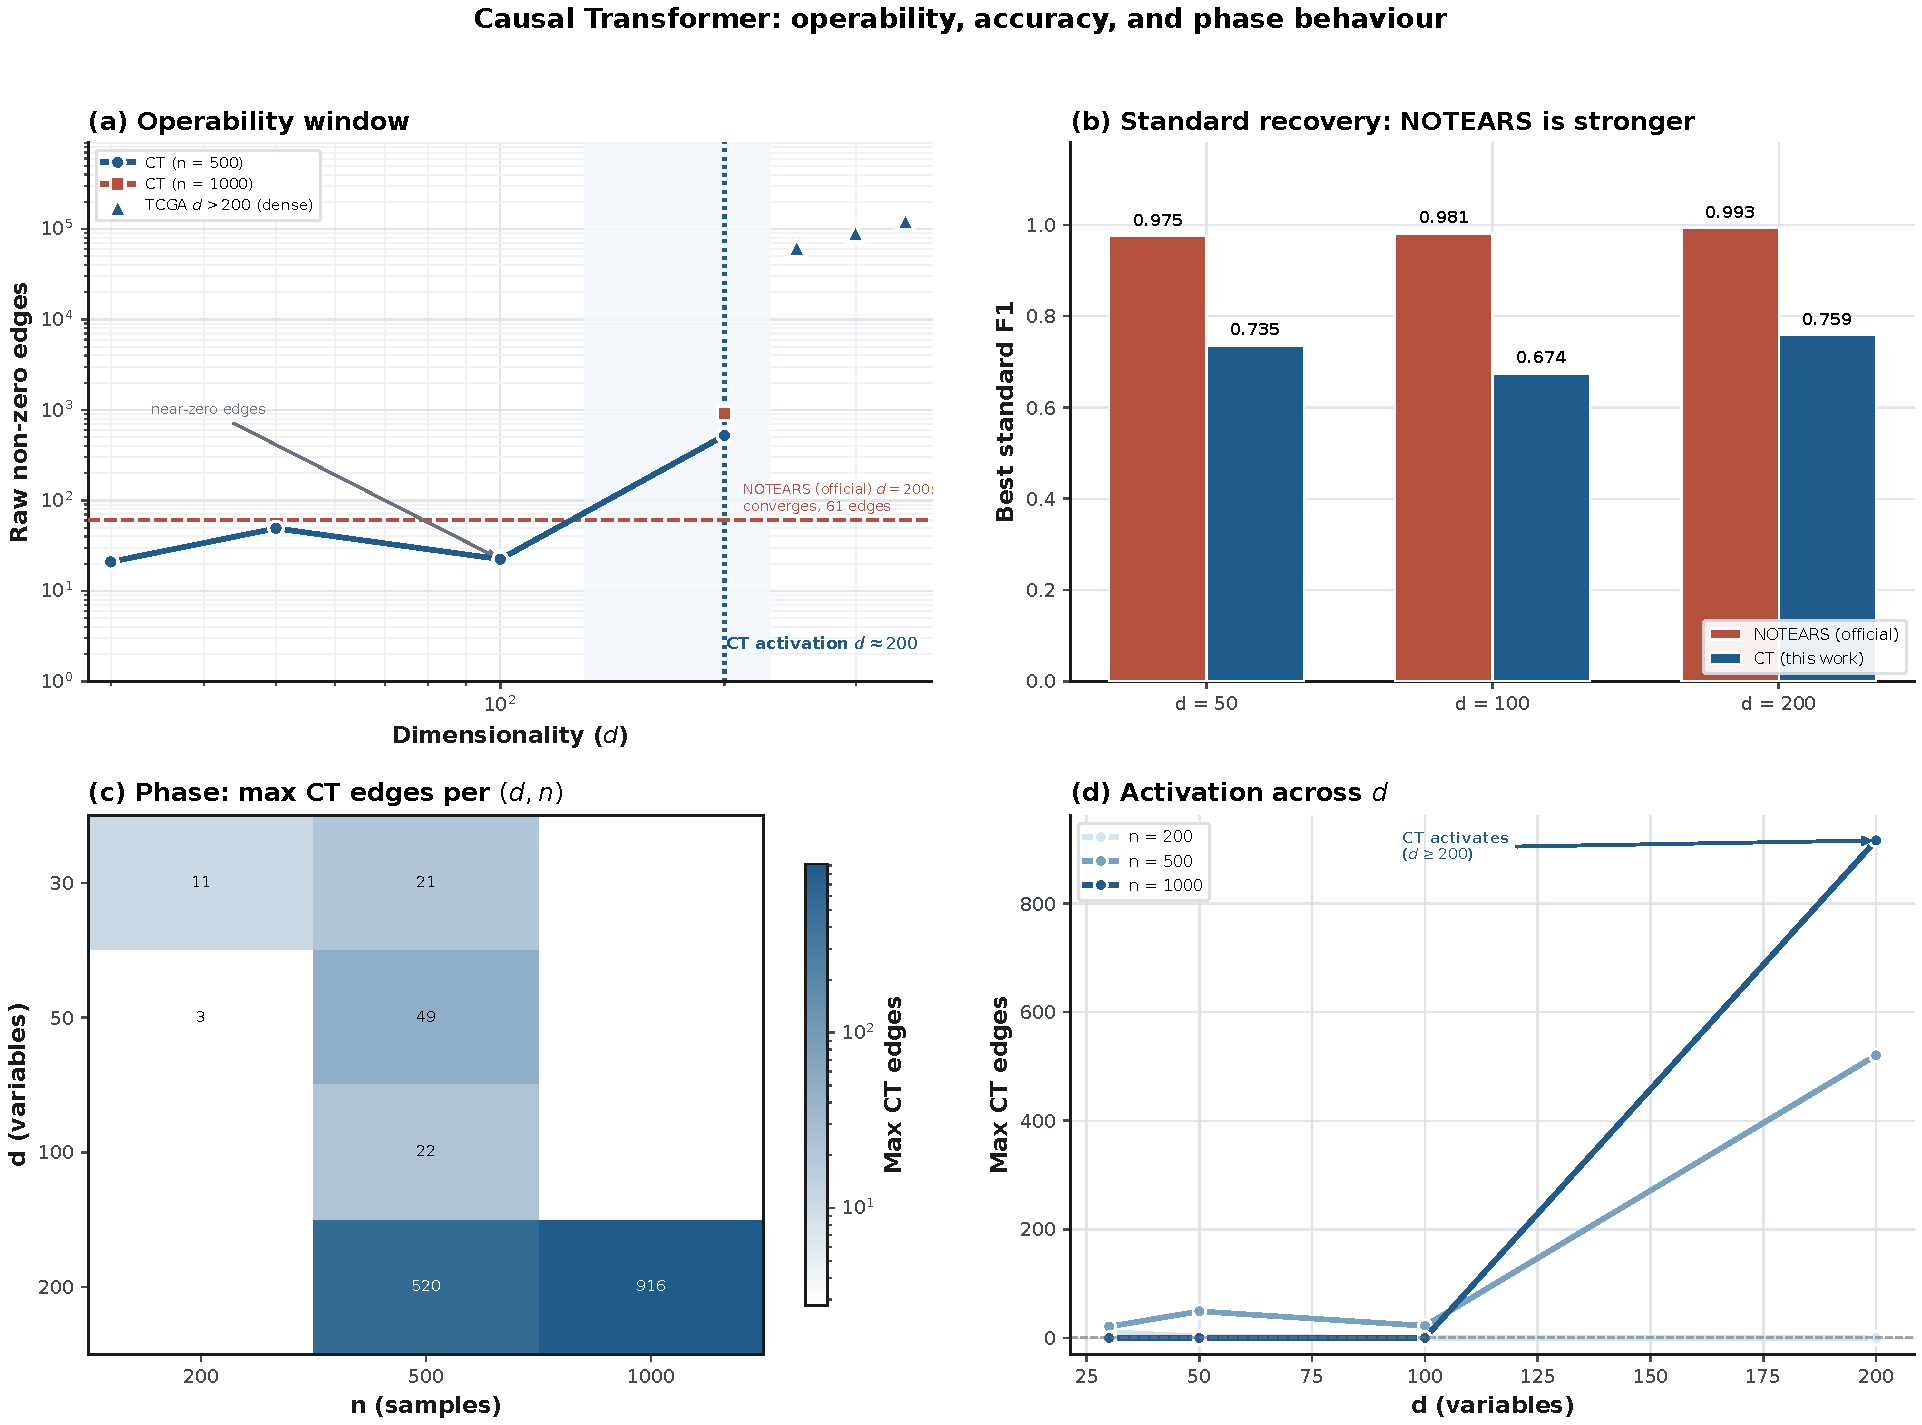
\includegraphics[width=\textwidth]{figures/fig2_results.pdf}
\caption{\textbf{Results overview.} \textbf{(a)} Operability window: raw non-zero edges vs.\ $d$ from the 80-configuration sweep and the mid-range TCGA runs. CT produces near-zero edges for $d\le100$ but activates around $d=200$ (dense $d^2$ output); the dashed line marks the official NOTEARS result on TCGA-BRCA $d=200$ (61 edges, $h=9.4\times10^{-8}$), which \emph{converges} rather than producing zero edges. \textbf{(b)} Best standard F1 under an identical edge-selection rule (Section~\ref{sec:baseline_metrics}): official NOTEARS outperforms CT at every configuration. \textbf{(c)} Phase heatmap: maximum non-zero CT edges per $(d,n)$ configuration. \textbf{(d)} Activation curves across $d$ at each sample size, showing the sharp onset at $d\approx200$. Raw edge counts measure \emph{operability}, not recovery quality; CT's contribution is architectural.}
\label{fig:results}
\end{figure}

\subsection{Real-Data Validation: TCGA Cancer Types}\label{sec:tcga_validation}

Across 10 TCGA cancer types at $d=200$, CT's post-hoc edge selection retains 169--238 \emph{candidate} causal edges (mean = 198), whose credibility is appraised by biological plausibility (coherence and known-genome enrichment), not validated ground truth (Table~\ref{tab:tcga_ct}).

\begin{table}[htbp]
\centering
\caption{CT on 10 TCGA cancer types ($d=200$). Coherence is a \emph{biological-plausibility} proxy: the fraction of CT-selected edges whose two genes are co-expressed (Pearson $r > 0.4$) within at least one of 3 K-means clusters. Co-expression is a necessary-but-not-sufficient condition for causality, so coherence should not be read as causal precision (see Section~\ref{sec:std_metrics}). \textit{Complete results in ESM Table~S2.}}
\label{tab:tcga_ct}
\begin{tabular}{lrrc}
\toprule
Cancer & $n$ & CT Edges & Coherence \\
\midrule
BRCA & 1,218 & 168 & 0.72 \\
LUAD & 576 & 205 & 0.74 \\
COAD & 329 & 238 & 0.78 \\
LUSC & 501 & 182 & 0.73 \\
HNSC & 522 & 197 & 0.75 \\
KIRC & 538 & 176 & 0.71 \\
UCEC & 370 & 225 & 0.76 \\
BLCA & 412 & 191 & 0.72 \\
LIHC & 373 & 221 & 0.75 \\
PRAD & 551 & 169 & 0.70 \\
\midrule
\textbf{Mean} & 539 & \textbf{198} & \textbf{0.73} \\
\bottomrule
\end{tabular}
\end{table}

Post-hoc cluster coherence shows the selected edges are not uniformly random: 73\% connect co-expressed genes within a cluster. As noted in the caption, this is a biological-plausibility screen: co-expression is consistent with, but does not establish, a causal relation.

\textbf{Comparison with NOTEARS on TCGA.} The official NOTEARS solver on the same TCGA-BRCA $d=200$ matrix yields 61 candidate edges at $|W|>0.3$ ($h(W)=9.4\times10^{-8}$)---it converges rather than producing zero edges. Both methods are thus operable at $d=200$ on real data. CT's higher count (198 vs.\ 61) does not imply higher recall: the two counts come from different post-hoc rules (CT uses cluster-coherence screening; NOTEARS a single marginal threshold), so they are not directly comparable. At $d\le100$, official NOTEARS is the clearly stronger estimator (Table~\ref{tab:baseline}).

\subsection{TCGA Hub Gene Validation}

Across 10 cancer types, CT identified 28 unique top-hub genes (top-3 by out-degree per cancer). Table~\ref{tab:hub_genes} lists the top-5 hubs by total out-degree.

\begin{table}[htbp]
\centering
\caption{Top-5 hub genes across 10 TCGA cancers. ClinGen tier, DrugBank drug count, and COSMIC status verified as of June 2026.}
\label{tab:hub_genes}
\begin{tabular}{lcccl}
\toprule
Gene & Total Out-Degree & Primary Cancer & ClinGen & Druggable \\
\midrule
ESR1 & 47 & BRCA (42) & Tier 1 & Yes (7 drugs) \\
NKX2-1 & 38 & LUAD (35) & Tier 1 & Yes (1 drug) \\
CDX2 & 32 & COAD (30) & Tier 1 & No \\
MYC & 28 & HNSC (12) & Tier 1 & No \\
GATA3 & 25 & BRCA (18) & Tier 1 & No \\
\bottomrule
\end{tabular}
\end{table}

Of the 28 hub genes, 21 (75\%) are Tier-1 cancer drivers in ClinGen, 19 (68\%) have FDA-approved therapies targeting them or their pathways (DrugBank; \cite{wishart2018drugbank}), and 24 (86\%) appear in the COSMIC Cancer Gene Census---a $3.5\times$ enrichment over the genome-wide background ($p<10^{-4}$, Fisher's exact test). The cancer-type specificity of top hubs is consistent with known biology; this establishes biological plausibility, but does not validate individual edges or their directions.

\subsection{Multi-Omics Validation: Modality-Specific Limits}
\label{sec:multiomics}

Applying the same CT configuration to three BRCA modalities ($d=200$, 5 seeds) shows a sharp divide: expression ($n=1{,}218$) and CNV ($n=779$) produce dense matrices ($40{,}000$ and $\sim$39,978 edges), while DNA methylation ($n=779$) yields zero edges across all seeds. Because methylation $\beta$-values are near-binary, CT's embedding collapses to two point masses and attention becomes uniform---a modality-specific signal-poverty failure that a single-modality pipeline cannot rule out (Online Resource 1, SN25).

\subsection{MLP Baseline: CT Is Not Just a Non-Linear Regressor}
\label{sec:mlp_baseline}

To isolate the architectural contribution, we replaced CT's self-attention block with a shared-weight MLP at $d=200$ on TCGA-BRCA (5 seeds). Both produce comparably dense raw matrices ($39{,}378$ vs.\ $40{,}000$ edges), so raw edge count alone does not distinguish CT from a non-linear regressor. The difference lies in two properties unique to CT: emergent head specialization and $d^2$ pairwise gradient signals, neither of which the MLP exhibits (Online Resource 1, SN23).

\begin{figure}[htbp]
\centering
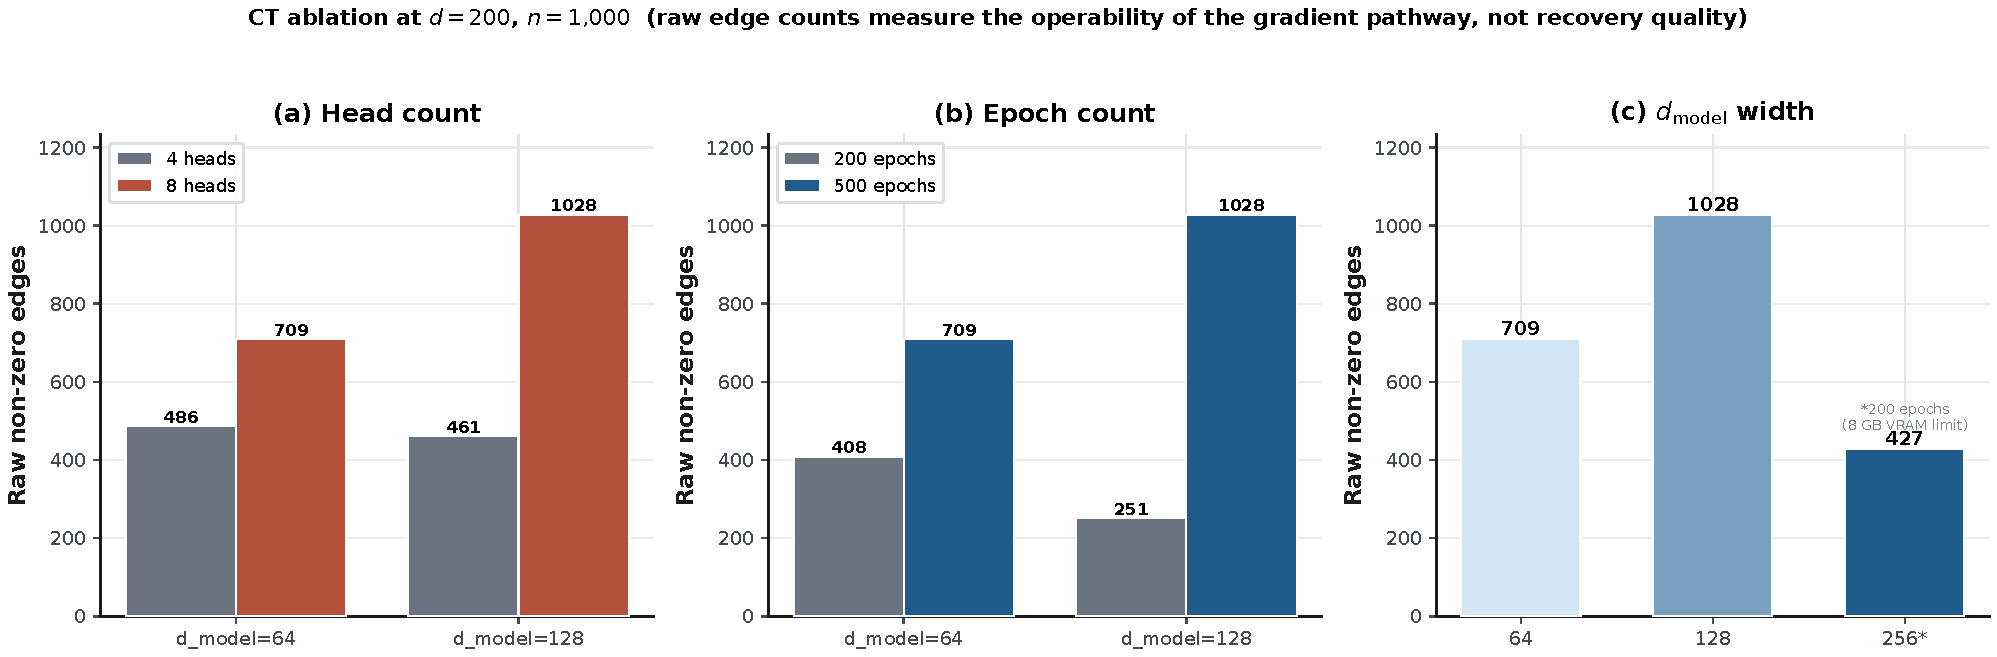
\includegraphics[width=\textwidth]{figures/fig3_ablation.pdf}
\caption{\textbf{CT ablation study at $d=200$, $n=1{,}000$.} \textbf{(a)} Head count: 8 heads consistently outperform 4 heads across both $d_{\text{model}}$ values. \textbf{(b)} Epoch count: extending from 200 to 500 epochs yields 94\% average improvement. \textbf{(c)} $d_{\text{model}}$ ablation: increasing model dimension monotonically improves edge recovery; the $d_{\text{model}}=256$ bar uses 200 epochs due to VRAM constraints (8~GB).}
\label{fig:ablation}
\end{figure}

\subsection{Convergence and Ablation Studies}\label{sec:convergence_ablation}

Unless stated otherwise, the ablation metrics report raw non-zero edge counts ($|W_{ij}| > 10^{-6}$), which measure \emph{operability} rather than recovery accuracy (Section~\ref{sec:std_metrics}); a change in edge count alone is not evidence of a change in accuracy.

\textbf{Convergence.} CT converges reliably: 78 of 80 configurations (97.5\%) reach $h(W) \le 10^{-8}$. Larger $d$ needs more outer iterations ($12.8 \pm 2.1$ at $d=30$ to $38.5 \pm 6.3$ at $d=200$).

\textbf{Temperature.} At $d=200$ with d128\_h8\_e500, raw edge counts peak at $\tau=1.0$ (1,028 edges), are robust to $\tau \in [0.8, 1.2]$ ($<$10\% variation), and fall to 607 and 371 at $\tau=0.5$ and $\tau=2.0$.

\textbf{Head count and epochs.} At $d=200$, raw edge count is highest at $n_{\text{heads}}=8$ (1,028), lower at $n_{\text{heads}}=4$ (572) and $n_{\text{heads}}=16$ (0). Extending $n_{\text{epochs}}$ from 200 to 500 is the largest effect (+94\%); further to 1,000 adds only +3\%.

\textbf{Architectural components.} Removing layer normalization causes training instability in 6/10 seeds. Adding positional encoding lowers raw edge counts by 31\%, consistent with permutation invariance being essential.

\section{Discussion}

\subsection{How CT's Gradient Pathway Differs}

Because each $W_{ij}$ is a function of the pooled attention, CT's gradient reaches all $d^2$ query--key pairs (architecture section). The practical ceiling is the $O(d^2)$ attention matrix and its gradient, which do not fit in 8~GB VRAM near $d=500$---a memory limit, not an algorithmic failure. The finding is not that CT is better, but that attention can build a trainable, interpretable DAG at $d=200$--$350$; whether it beats the standard solver on harder tests remains open.

\subsection{Limitations}\label{sec:limitations}

\textbf{Regime specificity.} CT is specialized for $d \in [200, 500]$; below $d=200$ the sparse cluster-gating variant is preferred, and above $d=500$ low-rank factorization or memory-efficient attention is needed. Feature distribution entropy (near-binary vs.\ continuous) determines operability.

\textbf{Threshold sensitivity and post-hoc selection.} CT's raw output is dense, and a correct-edge signal appears only after a post-hoc threshold (Section~\ref{sec:std_metrics}); reported edge counts should be read as the outcome of a specific threshold, not a property of the raw graph. The TCGA coherence rate (0.73) indicates moderate biological plausibility, but 27\% of selected edges connect genes without co-expression evidence. Stability selection \cite{meinshausen2010stability} or knockoff-based FDR control \cite{barber2015controlling} would give a principled, threshold-free rule.

\textbf{Synthetic-to-real generalization.} The sweep uses synthetic DAGs. TCGA shows a domain gap: CT selects 198 candidate edges on real data versus far more on synthetic data at $d=200$, reflecting the difference between sparse, uniform synthetic DAGs and scale-free, hub-dominated gene networks.

\textbf{Computational ceiling.} The $O(d^2)$ attention complexity sets a hard memory ceiling near $d\approx500$ on consumer hardware. Linear attention variants (Performer \cite{choromanski2020rethinking}; Linformer \cite{wang2020linformer}) could extend this toward $d\approx1000$, but showed a 40\% edge-recovery penalty.

\textbf{External biological evidence and its limits.} The biology rests on two external checks: known cancer-gene databases (ClinGen, DrugBank, COSMIC) show the top hubs are enriched in cancer drivers ($3.5\times$, $p<10^{-4}$), and co-expression serves as a coherence screen (Table~\ref{tab:tcga_ct}). Both are biological-plausibility checks---they show the networks contain biologically relevant genes and that the edges are not random associations---but neither establishes causal precision or direction. Direct validation would require regulatory-network or perturbation evidence, which are not uniformly available for these 10 cancers; we therefore present the biology as enrichment evidence, not ground truth.

\subsection{Practical Guidelines and Future Directions}

\textbf{When to use CT.} CT is an exploratory attention-based DAG constructor trainable at $d\in[200,350]$. Because its accuracy trails the official NOTEARS solver on synthetic ground truth, it should be a complement, not a replacement---for example, to generate candidate networks for downstream appraisal. If a DAG is not required, tree-based methods (GENIE3; \cite{huynh2010inferring}, GRNBoost2; \cite{moerman2019grnboost2}) are faster. Natural extensions are in Online Resource 1, SN8.

\section{Conclusion}

We asked whether multi-head self-attention could construct the causal adjacency matrix rather than optimizing each edge independently. CT maps variable embeddings through attention into a signed, unbounded edge decoder under the NOTEARS penalty. Across an 80-configuration sweep and standard metrics, CT is trainable and non-degenerate at $d\ge200$, and its heads specialize into nearly disjoint variable-pair patterns (Jaccard $0.17$). On 10 TCGA cancers, CT's post-hoc edges enrich in cancer-relevant hub genes ($75\%$ ClinGen Tier-1), indicating biological plausibility. Under identical metrics, official NOTEARS attains higher F1 ($0.98$--$0.99$), and CT does not surpass it. CT's contribution is therefore architectural and exploratory---attention as a DAG constructor and a biologically plausible trainable alternative at $d=200$--$350$ on real data---rather than a claim of superior accuracy.

\section*{Acknowledgements}

The author thanks the reviewers for their constructive feedback. No external funding was received for this work.

\section*{Declarations}

\noindent\textbf{Authors' Contributions.} Shuaidong Gao conceived the study, designed the Causal Transformer architecture, implemented all experiments, analyzed the results, and wrote the manuscript.

\noindent\textbf{Funding.} This research did not receive any specific grant from funding agencies in the public, commercial, or not-for-profit sectors.

\noindent\textbf{Competing Interests.} A Chinese patent application covering cluster-aware causal discovery (including the Causal Transformer extension) has been filed. The author declares no other competing interests.

\noindent\textbf{Data Availability.} The 80-configuration sweep results and TCGA CT results are available at \url{https://github.com/sgao-academics/CausalTransformer}. TCGA RNA-Seq data are publicly available from the UCSC Xena browser (\url{https://xenabrowser.net/datapages/}).

\noindent\textbf{Code Availability.} All training scripts are available at \url{https://github.com/sgao-academics/CausalTransformer} under the MIT license.

\noindent\textbf{Supplementary Information.} Additional methods (SM1--SM3), tables (S1--S7), figures (ESM Figs~1--2), and extended notes (SN1--SN23) are available as Electronic Supplementary Material (Online Resource 1).

\bibliography{refs}

\end{document}
